\section{待機をバックグラウンドに押しやる}

ほとんどのプログラムは、ファイル、ソケット、標準的なターミナルストリームを通して外部世界と接続します。これらすべてを入出力、I/Oと呼んでいます。最近のプロセッサは1秒間に何十億もの命令を実行することができますが、ほとんどのI/Oは比較的低速です。多くのプログラムは、ファイルからデータを読み込んだり、外部サーバーから応答を受け取ったり、ユーザーが何をしたいのかを調べるために、かなりの時間をかけて待機しています。

プログラムが他の作業を続けられるように、この待ち時間を効率的に処理する必要があります。待っている間、私たちは他の処理を行うこともできますし、複数の処理を並行して待つこともできます。例えば、ウェブブラウザは、外部のウェブサーバがコンテンツを返すのを待つと同時に、現在のページをレンダリングし、ユーザーがリンクをクリックしたりページをスクロールしたりするのに応答して時間を費やしているプログラムである。

\subsection{ファイヤー・アンド・フォーゲット}

まず、バックグラウンドで応答不要な作業を行うという単純なケースを考えてみよう。アプリケーションを構築しているときに、イベントが発生するたびに外部の計測器コレクターを呼び出したいとします。この外部サービスは、inc-stat という便利な関数でラップすることができます。更新するstatを指定して、この関数を呼び出します。


\begin{lstlisting}[numbers=none]
(inc-stat :pageview)
\end{lstlisting}

この関数は、ネットワーク経由で外部のウェブサービスを呼び出そうとしています。もし、ページビューを制作中に呼び出すと、次の図にあるように、その呼び出しにかかる時間は、ページを構築するごとに遅くなってしまいます。


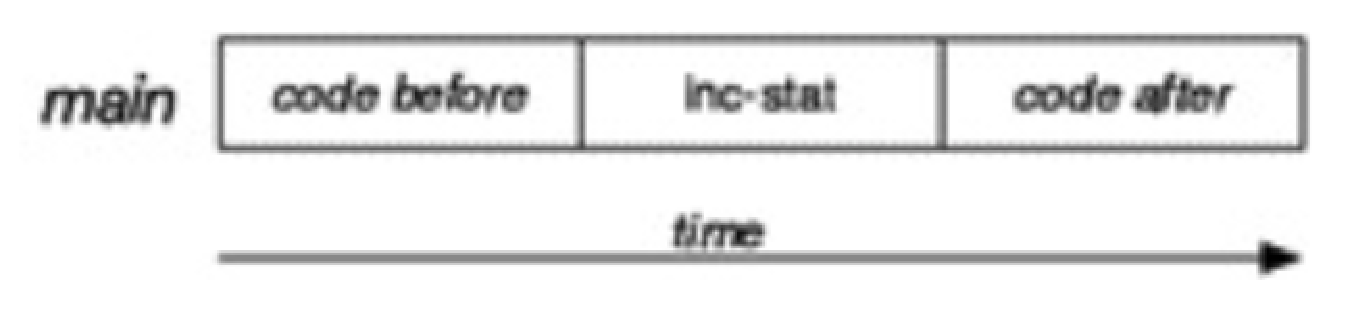
\includegraphics[width=10cm]{fig_05_001.eps}

この作業をバックグラウンドのスレッドに移すために、Clojureに含まれる\texttt{future}関数を使用します。

\begin{lstlisting}[numbers=none]
(future (inc-stat :pageview))
\end{lstlisting}

\texttt{future}関数はボディを受け取り、Clojure自身が維持するバックグラウンドのスレッドプールでそのボディを呼び出す。図にその違いを見ることができます。

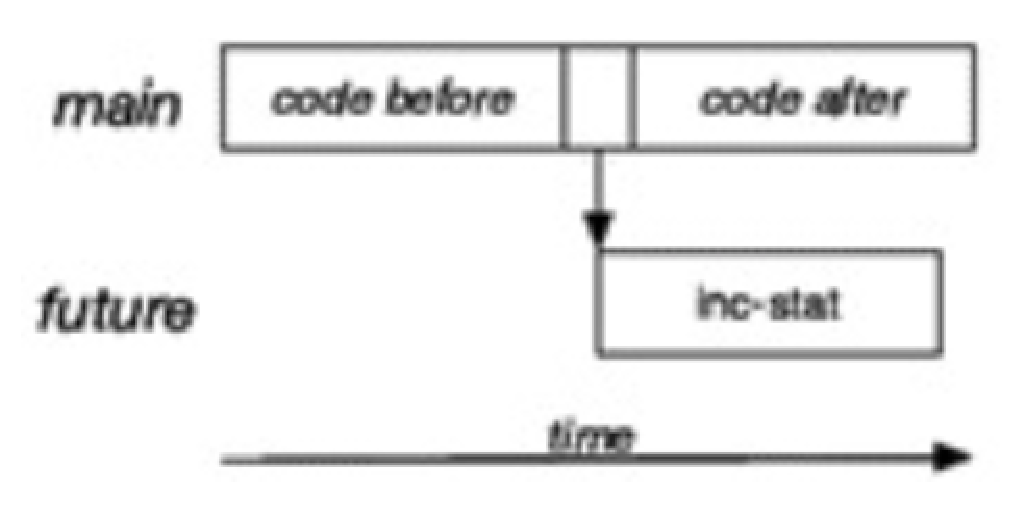
\includegraphics[width=8cm]{fig_05_002.eps}

また、\texttt{future-call}を使用すると、ボディを渡す代わりに引数のない関数を非同期で呼び出すことができます。どちらの関数も\texttt{java.lang.Future}オブジェクトを返し、それを使って非同期の活動を制御したり検査したりすることができます。\texttt{future-cancel}関数はその実行をキャンセルし、\texttt{future-done?}と\texttt{future-cancelled?}はその状態についての情報を与えてくれます。

しかし、独立した統計値増加メッセージをリモートサービスに大量に送信するのは非効率的だと思われます。送信前にいくつかのインクリメントメッセージをバッチ処理する方がより理にかなっています。そのためには、非同期かつステートフルである必要がある。


\subsection{非同期とステートフル}

第4章「状態、アイデンティティ、変化」では、Clojureの状態コンテナであるvar、atom、refを検討しました。もう一つの状態コンテナであるagentの紹介は、今まで遅らせました。

他のステート・コンテナと同様に、agentは不変の値を保持し、同じ更新モデルを使用して変更されます。他のコンテナとは異なり、agentは非同期に更新されます。

メトリクス・コレクターを考えてみましょう。ある統計量のカウンターをagentに保持することにしましょう。

\begin{lstlisting}[numbers=none]
(def pageview-stat (agent 0))
\end{lstlisting}

agentの更新ごとにリモートサービスを呼び出すのではなく、10回目の更新(agentの状態が10で割り切れる回数に達したとき)ごとに呼び出すことにします。これは、ウォッチ(すべてのステートコンテナで動作する)を使えば簡単にできます。


\begin{lstlisting}[numbers=none]
(add-watch
  pageview-stat
  :pageview
  (fn [key agent old new]
    (when (zero? (mod new 10))
      (remote-send key new))))
\end{lstlisting}

ここでは、\texttt{pageview-stat} エージェントに、その状態が変化したときに起動されるウォッチを追加しました。新しいエージェントの状態が 10 の倍数のときだけ外部サービスリクエストを発行するようにし、バッチ処理を行うようにしました。

そして、アプリケーションが使用するインクリメント関数を、エージェント上で非同期的に実行される関数として定義することができます。


\begin{lstlisting}[numbers=none]
(defn inc-stat [stat]
  (send-off stat inc))
\end{lstlisting}

Clojureは、agentに対して非同期で更新アクションを呼び出すための2つの関数、\texttt{send}と\texttt{send-off}を提供します。\texttt{send} は計算機的で I/O のためにブロックされないagentの更新のために使用します。基礎となるスレッドプールは、固定されたスレッドのセットを使用し、これらの更新が適時に完了することに依存します。\texttt{send-off} は、任意の時間ブロックされる可能性のある更新に使用します。基盤となるスレッドプール(futureにも使用)は必要に応じて拡張されるので、ブロックは問題にならない。\texttt{inc-stat}では、外部サービスを呼び出す可能性があるので(エージェントスレッドで実行されるwatchesを介して)、\texttt{send-off}を使用します。

agentの追加機能として、STM トランザクション内またはagentアクション自体の内部でagentに対して呼び出された \texttt{send} または \texttt{send-off} は、トランザクションが完了するまで遅延されます。これにより、agentは、STMトランザクション内(成功するために再試行する必要があるかもしれません)や、他のagentの更新アクション内から呼び出されて、副作用を発生させることが安全になります。

\begin{itembox}[l]{}シャットダウン
Javaでは、スレッドをデーモンスレッドとしてマークすることができます。JVMは、すべてのノンデーモンスレッドがその作業を完了したとき、優雅にシャットダウンします(一般的に、これはメイン起動スレッドが完了したときに起こります)。スレッドをデーモンスレッドとしてマークすることは、それがバックグラウンドワーカーであり、シャットダウンを妨げてはならないことを意味します。

 futureとagentアクションを処理するスレッドは、デーモンスレッドではありません。アプリケーションが期待通りに終了せず、ハングアップしているのを発見した場合、アプリケーションの終了時に \texttt{shutdown-agents} の呼び出しを追加する必要があると思われます。
\end{itembox}

これまでは、バックグラウンドでブロックするアクションを、レスポンスを使わずに実行してきました。ここでは、バックグラウンドのスレッドで行われた作業からどのようにレスポンスを受け取ることができるかを見てみましょう。

\subsection{レスポンス待ち}

時には、作業を後回しにし、後で結果を取りに来たいこともあります。例えば、ある商品を手に入れ、2つ以上のオンラインショップで価格を調べたい場合を考えてみましょう。このように、1つのスレッドで各店舗に順番に問い合わせをすることができます。

\begin{lstlisting}[numbers=none]
(defn query-stores [product stores]
  (for [store stores]
    (query store product)))
\end{lstlisting}

これを実行する時間は、次の図のように、各ストアに問い合わせる時間の合計となる。

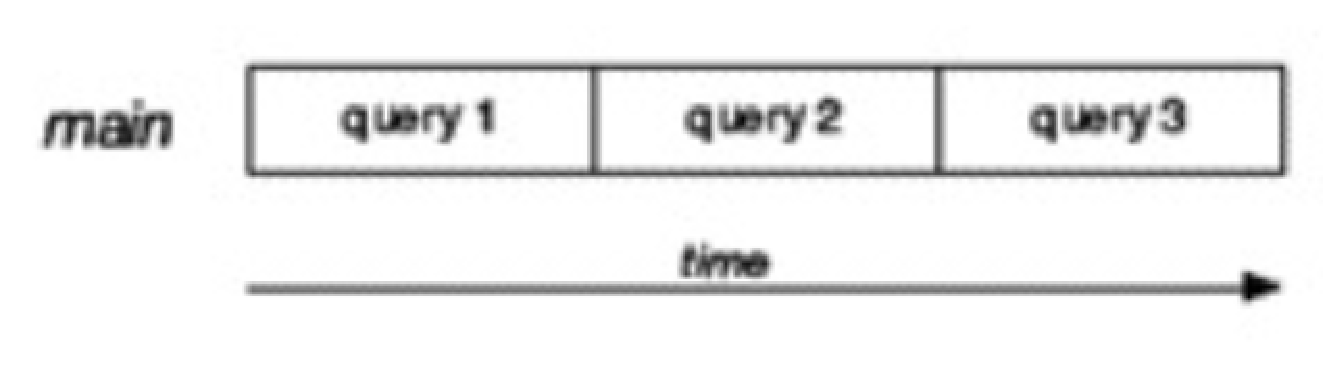
\includegraphics[width=10cm]{fig_05_003.eps}

もっといい方法があるはずだ! バックグラウンドスレッドに作業をプッシュする魔法のような機能を使えば、すべてのストアを同時にクエリすることができます。各非同期クエリにfutureを使用します。


\begin{lstlisting}[numbers=none]
(defn query-stores [product stores]
  (for [store stores]
    (future (query store product))))
\end{lstlisting}

しかし、先ほど述べたように、futureを呼び出すと\texttt{java.lang.Future}オブジェクトを返すので、\texttt{query-stores}は実際の結果ではなく、それらのシーケンスを返すようになりました。非同期呼び出しの結果をブロックして待つには、\texttt{deref} または短縮形の \texttt{@} を使って \texttt{Future} を再参照する必要があります。

\texttt{query-stores}関数は2段階で実装します。最初のステージは(既にある)全てのクエリを起動し、一連の\texttt{Future}オブジェクトを生成する。唯一の変更は、\texttt{doall}を呼び出すことで、クエリの起動を遅延させるのではなく熱心に行うようにすることです。もし\texttt{doall}を呼ばなければ、クエリは後でシーケンスが実現されるまで起動されません。第2ステージでは、それぞれの\texttt{Future}を参照し、それぞれが完了するまでブロックします。


\begin{lstlisting}[numbers=none]
(defn query-stores [product stores]
  (let [futures (doall
                  (for [store stores]
                    (future (query store product))))]
    (map deref futures)))
\end{lstlisting}

\texttt{query-stores}関数は、各ストアからの結果の遅延シーケンスを返す。また、futureをデリファレンスすることなく、遅延シーケンスを返すこともできます。この場合、呼び出し側は、各結果を解決するためにいつブロックするかを完全に制御することができます。

さて、クエリを同時に実行することで、次の図に示すように、複数のサービスを同時に待つことができ、より多くのスレッドを活用することで全体の時間を短縮することができます。この図では、3つのクエリストアがfutureで呼び出され、それぞれのクエリの結果をデリファレンスするために待機している様子を示しています。

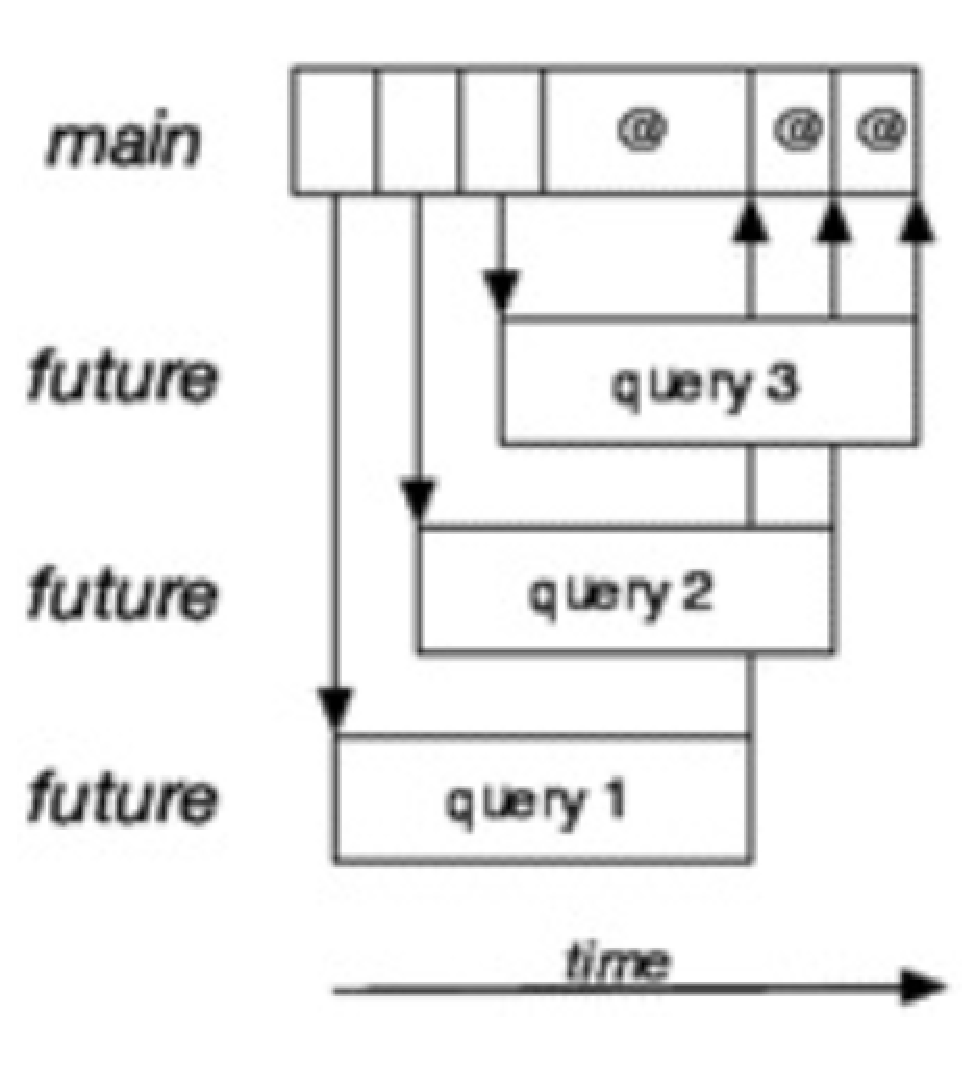
\includegraphics[width=10cm]{fig_05_004.eps}

この方法でfuturesを使用すると、1つの欠点があります。非同期の計算では、元のコードに1つの結果しか返せないのです。もし、計算の異なる時点で複数の値を返したい場合は、\texttt{promise}を使うことができます。

\subsection{プロミスの作成}

プロミスは1つのスレッドから別のスレッドに1つの値(そして1つだけ!)を転送するために使用されます。したがって、複数のプロミスは、非同期計算の異なる時間に値を返すために使用することができます。例えば、非同期計算の時間を計って、後でその実行の開始と終了の時間を取得したいとします。


\begin{lstlisting}[numbers=none]
(defn launch-timed []
  (let [begin-promise (promise)
        end-promise (promise)]
    (future (deliver begin-promise (System/currentTimeMillis))
      (long-running-task)
      (deliver end-promise (System/currentTimeMillis)))
    (println "task begin at" @begin-promise)
    (println "task end at" @end-promise)))
\end{lstlisting}

